% !TEX root = numb3rs.tex
\newpage
\subsection{407: Primacy}\label{407}

In this episode, Charlie suggests using an evolutionary algorithm to search for abnormal behavior after a murder occurs in a video game with a real-life component. Evolutionary algorithms imitate the biological process of natural selection to find optimal solutions. There is a notion of which potential solutions are ``fitter" than others. The fittest solutions survive as less fit solutions are weeded out; hopefully, resulting in very fit (optimal) solutions over time. On this page, we will see how a genetic algorithm (a particular kind of evolutionary algorithm) could conceivably be used with a satellite to find a point of maximal elevation on the Earth. Charlie explains: \\

\begin{center} ``Think of a pond. A pond is a healthy ecosystem where predator and prey are in balance. However, if an outside predator is introduced, well then the ecosystem changes. An evolutionary algorithm highlights abnormal alterations, it discerns subtle patterns, and locates the source of a problem.'' \end{center}

From this description, one might confuse the uses of evolutionary algorithms with the metaphor on which they are based. As we will see, abnormal alterations (mutations) occur in the execution of such algorithms. Presumably, Charlie has in mind a way of comparing behavior patterns and determining which actions are ``abnormal" for video game play. These will be the fittest for his purposes. In general, evolutionary algorithms can be potentially used anywhere there is a meaningful notion of ``fitness". This has nothing to do with searching for abnormal behavior. \\

\begin{figure}[H]
   \centering
   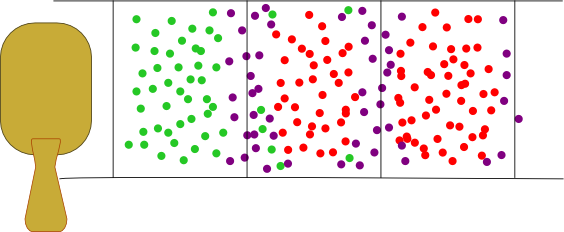
\includegraphics[width=2in]{111(4).jpg} 
\end{figure}

For instance, let's suppose we have a satellite that will tell us the elevation of the Earth at any specific longitude/latitude pair we ask of it. In this example, we are only allowed to ask the satellite to check one point at a time. One way of finding a high point is to ask the satellite to check (in some order) each point on a fine grid laid over the region, like a \bref{bitmap}{https://en.wikipedia.org/wiki/Bitmap} image. A genetic algorithm may be a more efficient approach. We define a longitude/latitude pair to be more ``fit" than another if it has a higher elevation. \\

\temph{Biology Review}

Before describing such a genetic algorithm in detail, let's first review the biology on which such algorithms are modeled. Biological traits (phenotype) of an organism are based in part on its DNA (genotype), which takes the form of a sequence of four different types of bases (A,C,G,T). Variation in genotype exists across a given population. Some individuals have genes that make them more likely than others to survive, reproduce, and produce fertile offspring. Such individuals are more ``fit". Fitness often depends on complicated relationships between various genes simultaneously present. Since fit organisms are more likely to pass their genes to the next generation, genes promoting fitness tend to become more prevalent with each successive generation. This process is known as natural selection.
\begin{figure}[H]
   \centering
   \includegraphics[width=3in]{huxley_evolution.jpg} 
\end{figure}

Various factors influence the natural selection process. Random mutations can occur in the genes of individual organisms. When these have any effect on fitness at all, it tends to be negative. Nonetheless, mutations can occasionally increase the fitness of an individual. Such mutations may become more prevalent in successive generations, by natural selection. Sexual reproduction, where the geneotype of offspring depends on the genotype of two parents, tends to lead to greater diversity of offspring than asexual reproduction, where offspring have a single parent. Population diversity, by virtue of a large number of gene combinations, may lead to the existence of some very fit individuals. (Diverse populations may also be better suited to surviving changes in how fitness is determined as environmental circumstances vary.) \\

\temph{Genetic Algorithm}

So how can we model an algorithm for our elevation problem on this biology? We already have a way of determining fitness -- points where the elevation is higher are more fit. We need a way of representing candidate longitude/latitude pairs as ``genetic" information. Instead of sequences of A,C,G,T, it is easier to work with sequences of 0's and 1's. One way of encoding our longitude/latitude pairs as such a string is to write both numbers in binary to some specified degree of precision (removing the decimal point), and then concatenate them (write one after the other to form a single string of 0's and 1's.) For instance, if our region is in the Northern and Western hemispheres, this encoding scheme is shown below. (Note: our organisms will only have a single chromosome, rather than pairs of them.) \\

\begin{figure}[H]
   \centering
   \includegraphics[width=3in]{encoding.png} 
\end{figure}

Now let's take an initial ``population." This is a collection of such strings as above, often chosen at random. For our particular genetic algorithm, we can choose to keep the population at a constant size, as follows. We will choose half the members of the population to reproduce by sexual reproduction, in pairs, each pair producing four offspring. At this point, the parents (and organisms that did not reproduce) ``die", and will be removed from the population. Such choices were somewhat arbitrary, and there are many similar algorithms. \\

In order to choose which half of the population reproduces, we could pair off individuals at random and let the more fit of each pair survive a given (large) proportion of the time, and the less fit survive the remainder of the time. Alternatively, we may wish to sort our population in order of fitness, letting the top third reproduce, ``killing" the bottom third, and giving individuals of the middle third a 50\% chance of reproduction. If we never allow the less fit organisms to reproduce, we might risk having low population diversity. \\

\begin{figure}[H]
   \centering
   \includegraphics[width=3in]{Morgan_crossover.jpg} 
\end{figure}

Now that we have chosen which individuals ``reproduce", we need to determine how their genetic information is combined. One easy way of doing this is based on an actual biological process: \bref{crossing over of chromosomes}{https://en.wikipedia.org/wiki/Chromosomal_crossover}. For each pair of reproducing individuals, choose a random position in the genetic string. Now, swap the portions of the two parents' chromosomes after this position, and we have two offspring with genes based on, but (usually) not the same as either parent. Swapping at a different point, the same parents produce a second pair of offspring. \\

\begin{figure}[H]
   \centering
   \includegraphics[width=3in]{parent.png} 
\end{figure}

Finally, we would like to add some mutations to our population in hopes of potentially finding some fitter individuals. Choose some specific (small) number p. Now, look at each bit (0 or 1) of each string in the population, and change it to its opposite (1 or 0) with probability $p$. Now we have \bref{the next generation}{http://www.math.cornell.edu/~numb3rs/baker/tng.jpg}! Repeating the process of selection, reproduction, and mutation for many generations, the genetic algorithm will hopefully produce a population with high fitness, and give us good solutions to our problem. \\












